% PROPOSAL 1 for the bottom row (compact: narrow (c), wide (d), shorter row); generated from fig_pipeline_v0_current.tex. Bars and dots are illustrative.
% Pipeline figure (main text), drawn at final print width 16.5 cm.
% Example: Electricity task wu2025:plan_choice:p06_p32_o6, as rendered by code/data/base.py:make_view.
% Inline tokens are the role names from code/kev/kev/model.py:encode (reserved tokenizer tokens in the code);
% the pointer head is PointerHead (formula in the Web Appendix).
% Equation numbers refer to manuscript-training.qmd: (2) eq-resp-ce, (3) eq-pop-ols, (4) eq-eval-mse.
% Build: pdflatex fig_pipeline.tex && pdftoppm -png -r 300 -singlefile fig_pipeline.pdf fig_pipeline
\documentclass[tikz,border=2pt]{standalone}
% Shared look for the pipeline figures. Sizes are final print sizes (no scaling in the manuscript).
% Colors: Okabe-Ito. Blue = model prediction, vermilion = trainable theta, dark gray = human / data.
\usepackage[T1]{fontenc}
\usepackage{lmodern}
\usepackage{amsmath,amssymb,bm}
\usepackage{array}
\renewcommand{\familydefault}{\sfdefault}
\usetikzlibrary{positioning,arrows.meta,calc,fit,backgrounds}
\pgfdeclarelayer{back}\pgfsetlayers{back,background,main}

\definecolor{cpred}{HTML}{0072B2}
\definecolor{ctrain}{HTML}{D55E00}
\definecolor{chuman}{HTML}{333333}
\definecolor{cline}{HTML}{555555}
\definecolor{cfield}{HTML}{F2F2F2}
\definecolor{cframe}{HTML}{BBBBBB}
\definecolor{ctok}{HTML}{007A5A}  % Okabe-Ito bluish green, darkened: special tokens

\tikzset{
  >={Stealth[length=3.5pt]},
  every node/.append style={execute at begin node={\hyphenpenalty=10000\exhyphenpenalty=10000}},
  flow/.style={->, line width=0.6pt, draw=cline},
  pred/.style={->, line width=0.9pt, draw=cpred},
  grad/.style={->, line width=0.8pt, draw=ctrain, dash pattern=on 3pt off 2pt},
  panel/.style={draw=cframe, line width=0.5pt, rounded corners=3pt},
  ptitle/.style={font=\footnotesize\bfseries, anchor=north west, inner sep=0pt},
  raw/.style={draw=cframe, fill=white, rounded corners=1.5pt, font=\scriptsize, align=left, inner sep=2.5pt},
  field/.style={draw=cline, fill=cfield, rounded corners=1.5pt, font=\scriptsize, align=left, inner sep=2.5pt},
  box/.style={draw=cline, fill=white, rounded corners=2pt, align=center, font=\footnotesize, inner sep=2.5pt},
  predbox/.style={box, draw=cpred, line width=0.8pt},
  humanbox/.style={box, draw=chuman, line width=0.8pt},
  trainbox/.style={box, draw=ctrain, line width=0.9pt},
  rawtxt/.style={raw, draw=none, fill=none},
  fieldtxt/.style={field, draw=none, fill=none},
  note/.style={font=\scriptsize, text=black!70, align=left, inner sep=0pt, anchor=north west},
}
\newcommand{\tok}[1]{\textcolor{ctok}{\textbf{\texttt{#1}}}}
% \rowboxes{raw node}{field node}{bottom coordinate}: draws both boxes down to the lower of the two bottoms,
% so a raw item and its input field always have the same height, and links them with an arrow at mid-height.
\newcommand{\rowboxes}[3]{%
  \path let \p1=(#1.south), \p2=(#2.south), \n1={min(\y1,\y2)} in coordinate (#3) at (0,\n1);
  \begin{scope}[on background layer]
    \draw[raw]   (#1.north west) rectangle (#1.east |- #3);
    \draw[field] (#2.north west) rectangle (#2.east |- #3);
  \end{scope}
  \coordinate (#3-mid) at ($(#1.north east)!0.5!(#1.east |- #3)$);
  \draw[flow] (#3-mid) -- (#3-mid -| #2.west);
}


\begin{document}
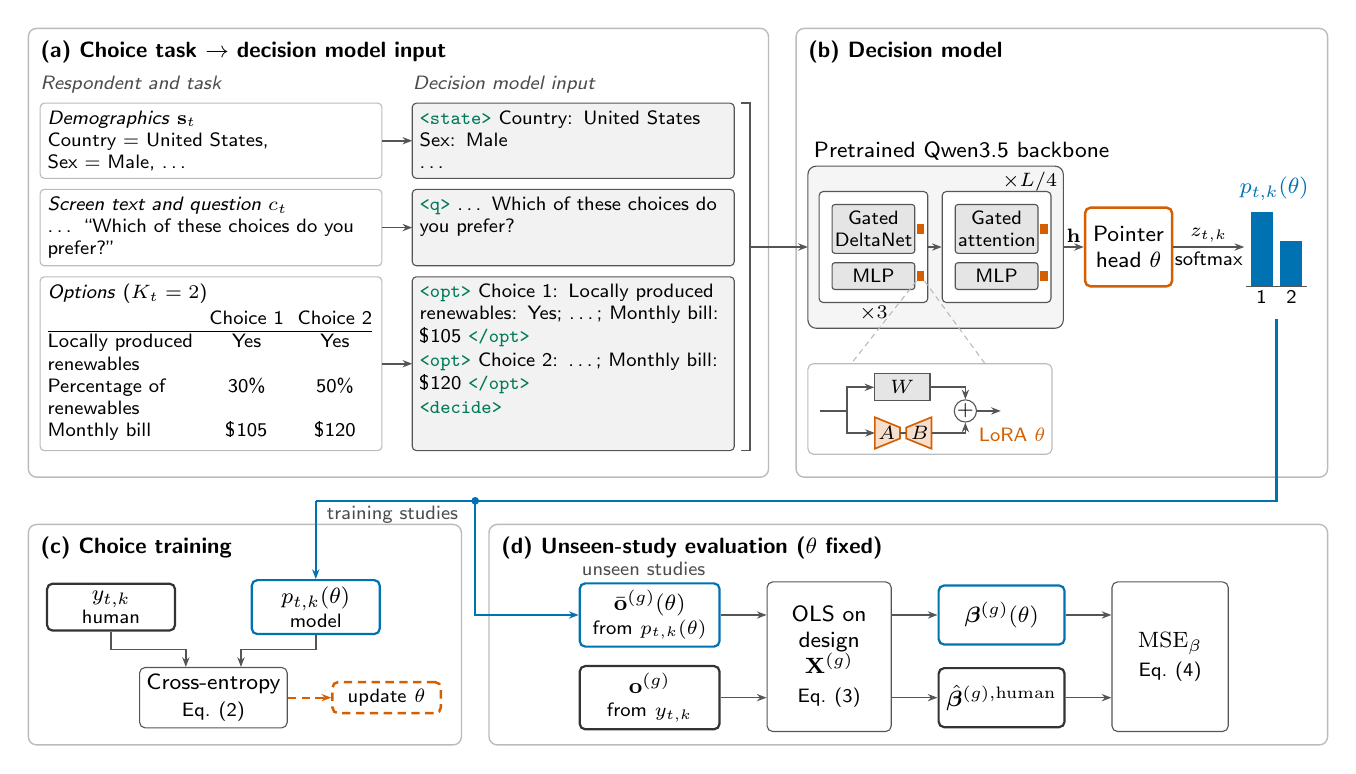
\begin{tikzpicture}

% ---------------------------------------------------------------- frames
\draw[panel] (0,0) rectangle (9.4,-5.7);
\draw[panel] (9.75,0) rectangle (16.5,-5.7);
\draw[panel] (0,-6.3) rectangle (5.5,-9.1);
\draw[panel] (5.85,-6.3) rectangle (16.5,-9.1);

\node[ptitle] at (0.15,-0.15) {(a) Choice task $\rightarrow$ decision model input};
\node[ptitle] at (9.9,-0.15) {(b) Decision model};
\node[ptitle] at (0.15,-6.45) {(c) Choice training};
\node[ptitle] at (6.0,-6.45) {(d) Unseen-study evaluation ($\theta$ fixed)};

% ================================================================ (a)
\node[note, font=\scriptsize\itshape] at (0.15,-0.6) {Respondent and task};
\node[note, font=\scriptsize\itshape] at (4.88,-0.6) {Decision model input};

\coordinate (inx) at (6.92,0);
\node[rawtxt, text width=4.15cm, anchor=north west] (rs) at (0.15,-0.95) {%
  \textit{Demographics} $\mathbf{s}_t$\\
  Country = United States,\\ Sex = Male, \ldots};
\node[fieldtxt, text width=3.9cm, anchor=north] (fs) at (rs.north -| inx) {%
  \tok{<state>} Country: United States\\
  Sex: Male\\
  \ldots};
\rowboxes{rs}{fs}{b1}

\node[rawtxt, text width=4.15cm, anchor=north west] (ri) at ($(b1)+(0.15,-0.14)$) {%
  \textit{Screen text and question} $c_t$\\
  \ldots\ ``Which of these choices do you prefer?''};
\node[fieldtxt, text width=3.9cm, anchor=north] (fi) at (ri.north -| inx) {%
  \tok{<q>} \ldots\ Which of these choices do you prefer?};
\rowboxes{ri}{fi}{b2}

\node[rawtxt, text width=4.15cm, anchor=north west] (rc) at ($(b2)+(0.15,-0.14)$) {%
  \textit{Options} ($K_t = 2$)\\[1pt]
  \begin{tabular}{@{}>{\raggedright\arraybackslash}p{1.95cm}@{\hspace{3pt}}c@{\hspace{5pt}}c@{}}
                              & Choice 1 & Choice 2 \\ \hline
  Locally produced renewables & Yes   & Yes   \\
  Percentage of renewables    & 30\%  & 50\%  \\
  Monthly bill                & \$105 & \$120 \\
  \end{tabular}};
\node[fieldtxt, text width=3.9cm, anchor=north] (fc) at (rc.north -| inx) {%
  \tok{<opt>} Choice 1: Locally produced renewables: Yes; \ldots; Monthly bill: \$105 \tok{</opt>}\\[1pt]
  \tok{<opt>} Choice 2: \ldots; Monthly bill: \$120 \tok{</opt>}\\[1pt]
  \tok{<decide>}};
\rowboxes{rc}{fc}{b3}

% ================================================================ (b)
% Qwen3.5 backbone (configs of Qwen3.5-0.8B/4B/9B): a 4-layer block repeated L/4 times
% (L = 24 or 32): 3 x [Gated DeltaNet + MLP], then 1 x [gated full attention + MLP].
% LoRA adapts every linear map in these modules (code/kev/kev/model.py, lora_targets="all").
% Vertical layout: the group (label .. zoom) is centred in the panel interior (-0.45 .. -5.7).
\coordinate (bbtop) at (9.9,-1.75);
\tikzset{
  layerbox/.style={draw=cline, fill=white, rounded corners=1.5pt, inner sep=0pt},
  mixer/.style={draw=cline, fill=black!10, rounded corners=1pt, align=center, font=\scriptsize,
                text width=0.98cm, minimum height=0.62cm, inner sep=1pt},
  mlp/.style={draw=cline, fill=black!10, rounded corners=1pt, align=center, font=\scriptsize,
              text width=0.98cm, minimum height=0.34cm, inner sep=1pt},
}
\newcommand{\loratab}[1]{\fill[ctrain] ($(#1.east)+(0.015,-0.06)$) rectangle ($(#1.east)+(0.115,0.06)$);}

\node[mixer, anchor=north west] (m1) at ($(bbtop)+(0.3,-0.48)$) {Gated\\DeltaNet};
\node[mlp, below=3pt of m1] (f1) {MLP};
\node[mixer, anchor=north west] (m2) at ($(m1.north east)+(0.5,0)$) {Gated\\attention};
\node[mlp, below=3pt of m2] (f2) {MLP};
\foreach \n in {m1,f1,m2,f2} { \loratab{\n} }
\begin{scope}[on background layer]
  \node[layerbox, fit=(m1)(f1), inner sep=4.5pt] (L1) {};
  \node[layerbox, fit=(m2)(f2), inner sep=4.5pt] (L2) {};
\end{scope}
\node[font=\scriptsize, anchor=north, inner sep=1pt] at (L1.south) {$\times 3$};
\draw[flow] (L1.east) -- (L2.west);
\coordinate (bbse) at ($(L2.south east)+(0.15,-0.32)$);
\begin{pgfonlayer}{back}
  \draw[draw=cline, fill=black!4, rounded corners=3pt] (bbtop) rectangle (bbse);
\end{pgfonlayer}
\node[font=\scriptsize, anchor=north east, inner sep=2pt] at (bbtop -| bbse) {$\times L/4$};
\coordinate (bbW) at (bbtop |- L1.west);
\coordinate (bbE) at (bbse |- L1.west);
\node[font=\footnotesize, anchor=south west, inner sep=2pt] at (bbtop) {Pretrained Qwen3.5 backbone};

% bracket: the three boxes are one input sequence; one arrow into the backbone
\draw[cline, line width=0.6pt] ($(fs.north east)+(0.08,0)$) -- ++(0.12,0) |- ($(fs.east |- b3)+(0.08,0)$);
\draw[flow] ($(fs.east |- bbW)+(0.2,0)$) -- (bbW);

% zoom: every linear map in the backbone is W + BA (LoRA)
\coordinate (lc) at ($(bbtop |- bbse)+(0.05,-1.05)$);
\draw[draw=cframe, rounded corners=2pt] ($(lc)+(-0.05,0.6)$) rectangle ($(lc)+(3.05,-0.55)$);
\draw[cframe, dash pattern=on 2pt off 1.5pt] ($(f1.east)+(0.015,-0.06)$) -- ($(lc)+(0.5,0.6)$);
\draw[cframe, dash pattern=on 2pt off 1.5pt] ($(f1.east)+(0.115,-0.06)$) -- ($(lc)+(2.2,0.6)$);
\node[draw=cline, fill=black!10, minimum width=0.7cm, minimum height=0.34cm, inner sep=0pt, font=\scriptsize] (W)
  at ($(lc)+(1.15,0.3)$) {$W$};
\draw[draw=ctrain, fill=ctrain!20, line width=0.6pt] ($(lc)+(0.8,-0.08)$) -- ($(lc)+(1.12,-0.21)$) -- ($(lc)+(1.12,-0.35)$) -- ($(lc)+(0.8,-0.48)$) -- cycle;
\draw[draw=ctrain, fill=ctrain!20, line width=0.6pt] ($(lc)+(1.2,-0.21)$) -- ($(lc)+(1.52,-0.08)$) -- ($(lc)+(1.52,-0.48)$) -- ($(lc)+(1.2,-0.35)$) -- cycle;
\node[font=\scriptsize, inner sep=0pt] at ($(lc)+(0.95,-0.28)$) {$A$};
\node[font=\scriptsize, inner sep=0pt] at ($(lc)+(1.37,-0.28)$) {$B$};
\node[draw=cline, circle, inner sep=0pt, minimum size=0.22cm, font=\scriptsize] (plus) at ($(lc)+(1.95,0)$) {$+$};
\draw[cline, line width=0.5pt] ($(lc)+(0.1,0)$) -- ($(lc)+(0.45,0)$) coordinate (split);
\draw[flow] (split) |- (W.west);
\draw[flow] (split) |- ($(lc)+(0.8,-0.28)$);
\draw[cline, line width=0.5pt] ($(lc)+(1.12,-0.28)$) -- ($(lc)+(1.2,-0.28)$);
\draw[flow] (W.east) -| (plus.north);
\draw[flow] ($(lc)+(1.52,-0.28)$) -| (plus.south);
\draw[flow] (plus.east) -- ($(lc)+(2.4,0)$);
\node[font=\scriptsize, text=ctrain, anchor=west, inner sep=1pt] at ($(lc)+(2.08,-0.3)$) {LoRA $\theta$};

% pointer head and predicted probabilities, aligned with the backbone row
\node[trainbox, text width=0.93cm, minimum height=1.0cm, anchor=west] (ph) at ($(bbE)+(0.26,0)$)
  {Pointer head $\theta$};
\draw[flow] (bbE) -- (ph.west) node[midway, above, font=\scriptsize, inner sep=1.5pt] {$\mathbf{h}$};

\coordinate (pb) at ($(ph.east)+(0.98,-0.5)$);
\foreach \i/\h/\lab in {0/0.95/1, 1/0.58/2} {
  \fill[cpred] ($(pb)+(0.38*\i,0)$) rectangle ($(pb)+(0.38*\i+0.28,\h)$);
  \node[font=\scriptsize, below, inner sep=1.5pt] at ($(pb)+(0.38*\i+0.14,0)$) {\lab};
}
\draw[cline, line width=0.4pt] ($(pb)+(-0.06,0)$) -- ($(pb)+(0.72,0)$);
\node[font=\footnotesize, text=cpred, anchor=south east, inner sep=1pt] at ($(pb)+(0.78,1.05)$) {$p_{t,k}(\theta)$};
\draw[flow] (ph.east) -- ($(ph.east)+(0.9,0)$)
  node[midway, above, font=\scriptsize, inner sep=1.5pt] {$z_{t,k}$}
  node[midway, below, font=\scriptsize, inner sep=1.5pt] {softmax};

% ================================================================ (c)  [option 1: compact]
\node[humanbox, text width=1.45cm] (cy) at (1.05,-7.35) {$y_{t,k}$\\[-1pt]{\scriptsize human}};
\node[predbox, text width=1.45cm] (cp) at (3.65,-7.35) {$p_{t,k}(\theta)$\\[-1pt]{\scriptsize model}};
\node[box, text width=1.7cm] (ce) at (2.35,-8.5) {Cross-entropy\\{\scriptsize Eq.~(2)}};
\node[trainbox, text width=1.2cm, dash pattern=on 3pt off 2pt] (upd) at (4.55,-8.5) {\scriptsize update $\theta$};
\draw[flow] (cy.south) |- ($(ce.north)+(-0.35,0.22)$) -- ($(ce.north)+(-0.35,0)$);
\draw[flow] (cp.south) |- ($(ce.north)+(0.35,0.22)$) -- ($(ce.north)+(0.35,0)$);
\draw[grad] (ce.east) -- (upd.west);

% ================================================================ (d)
\node[predbox, text width=1.6cm] (ob) at (7.89,-7.45) {$\bar{\mathbf{o}}^{(g)}(\theta)$\\[-1pt]{\scriptsize from $p_{t,k}(\theta)$}};
\node[humanbox, text width=1.6cm] (oh) at (7.89,-8.5) {$\mathbf{o}^{(g)}$\\[-1pt]{\scriptsize from $y_{t,k}$}};
\node[box, text width=1.4cm, minimum height=1.9cm] (ols) at (10.17,-7.98) {OLS on design $\mathbf{X}^{(g)}$\\[1pt]{\scriptsize Eq.~(3)}};
\node[predbox, minimum width=1.6cm, minimum height=0.75cm] (bm) at (12.36,-7.45) {$\boldsymbol{\beta}^{(g)}(\theta)$};
\node[humanbox, minimum width=1.6cm, minimum height=0.75cm] (bh) at (12.36,-8.5) {$\hat{\boldsymbol{\beta}}^{(g),\mathrm{human}}$};
\node[box, text width=1.3cm, minimum height=1.9cm] (mse) at (14.5,-7.98) {$\mathrm{MSE}_\beta$\\[1pt]{\scriptsize Eq.~(4)}};
\draw[flow] (ob.east) -- (ob.east -| ols.west);
\draw[flow] (oh.east) -- (oh.east -| ols.west);
\draw[flow] (bm.west -| ols.east) -- (bm.west);
\draw[flow] (bh.west -| ols.east) -- (bh.west);
\draw[flow] (bm.east) -- (bm.east -| mse.west);
\draw[flow] (bh.east) -- (bh.east -| mse.west);
\node[font=\scriptsize, text=black!70, anchor=south west, inner sep=1pt] at ($(ob.north west)+(0,0.04)$) {unseen studies};

% ================================================================ prediction bus: (b) -> (c), (d)
\coordinate (pdrop) at ($(pb)+(0.33,-0.42)$);
\draw[line width=0.9pt, draw=cpred] (pdrop) |- (cp.north |- 0,-6.0) coordinate (bus-l);
\draw[pred] (bus-l) -- (cp.north);
\coordinate (bj) at (5.675,-6.00);
\fill[cpred] (bj) circle (1.4pt);
\draw[pred] (bj) |- (ob.west);
\node[font=\scriptsize, text=black!70, anchor=north west, inner sep=1pt] at ($(cp.north |- 0,-6.0)+(0.1,-0.03)$) {training studies};
\end{tikzpicture}
\end{document}
